\documentclass[10pt, a4paper]{article}
\usepackage{lrec2016}
% \usepackage{multibib}
% \newcites{languageresource}{Language Resources}
\usepackage{graphicx}
\usepackage{amssymb,amstext,amsmath,amsthm}
\usepackage{epstopdf}
\usepackage[latin1]{inputenc}
 \usepackage{hyphenat}
\hyphenation{lexico-graphy}

% To include:

% ERROR ANALYSIS 
% babelnet_dir = "/Users/alex/tmp/matching/babelnet/"
% adagram_fpath = "/Users/alex/tmp/matching/ddt-adagram-ukwac+wacky.csv.gz.voc.out"


\title{Best of Both Worlds: Making Word Sense Embeddings Interpretable}

\name{Alexander Panchenko}

\address{  Language Technology Group, Technische Universit\"at Darmstadt \\
Hochschulstr. 10, 64289, Darmstadt, Germany \\
              panchenko@lt.informatik.tu-darmstadt.de\\}


\abstract{Word sense embeddings represent a word sense as a low-dimensional numeric vector. While this representation is potentially useful for NLP applications, its interpretability is inherently limited. We propose a simple technique that improves interpretability of sense vectors by mapping them to synsets of a lexical resource. Our experiments with AdaGram sense embeddings and BabelNet synsets show that it is possible to retrieve synsets that correspond to automatically learned sense vectors with Precision of 0.87, Recall of 0.42 and AUC of 0.78. \\ \newline \Keywords{word sense embeddings, WordNet, BabelNet, AdaGram, sense matching, lexical semantics}}



\begin{document}

\maketitleabstract

\section{Introduction}

 
Two main approaches to represent the meaning of lexical units, such as words and multiword expressions are lexico\-graphy and statistical corpus analysis. In the first approach, a human explicitly encodes lexical-semantic knowledge, usually in the form of synsets (i.e. sets of synonyms),
typed relations between synsets and sense definitions. A prominent example of this approach is the Princeton WordNet~\cite{miller1995wordnet}. The second approach makes use of text corpora to extract relations between words and feature representations of words and senses. These methods are trying to avoid manual work as much as possible. Whereas lexical resources are manually created, in the second approach most methods extract the information from text without human intervention. Examples of the second group of methods include "classical" vector-based~\cite{baroni2010distributional} and symbolic~\cite{Biemann2013} distributional models, as well as word embeddings~\cite{mikolov2013efficient,pennington2014glove}.

One of the strongest sides of lexical-semantic resources is their \textit{interpretability} -- they are entirely human-readable and drawn distinctions are motivated by lexicographic or psychological considerations. On the downside,  these WordNet-like resources are expensive to create, and it is not easy to adapt them to a given domain of interest or language. Besides, sense inventories of lexical resources are often too fine grained to be useful in downstream applications~\cite{brown2008choosing}.

At the same time, corpus-driven approaches are strong at \textit{adaptivity} -- they can be re-trained on a new corpus, thus naturally adapting to the domain at hand. If fitted with a word sense induction algorithm, corpus-driven approaches can also discover new senses \cite{erkEtAl2009}. However, the representations they deliver are often not matching the standards of lexicography, and they rather distinguish word usages than senses. Moreover, dense numeric vector representations as present in latent vector spaces \cite{Schutze1998} and word embeddings are barely interpretable.

Word sense embeddings~\cite{Huang2012,tianEtAl2014,neelakantanefficient} extend word embeddings so that a word is represented by several vectors corresponding to meanings of the word. Li and Jurafsky~\shortcite{li2015multi} show that sense embeddings can significantly improve performance of part-of-speech tagging, semantic relation identification and semantic relatedness tasks, but yield no improvement for named entity recognition and sentiment analysis. Sense embeddings suffer the same interpretability limitations as other dense vector representations.  


The contribution of the paper is a technique that links word sense embeddings to a lexical resource, making them more interpretable. The main motivation of the technique is to close the gap between interpretability and adaptivity of lexical-semantic models. We demonstrate the performance of our method by linking AdaGram sense embeddings, proposed by Bartunov et  al.~\shortcite{bartunov2015breaking} to synsets of BabelNet~\cite{navigli2010babelnet}. However, the approach can be straightforwardly applied to any combination of a WordNet-like resource and a word sense embeddings model. Scripts and datasets related to this experiment are available online.\footnote{http://tudarmstadt-lt.github.io/vec2synset}


 To our knowledge, this is the first attempt to tag sense embeddings with interpretable synsets from a lexical resource. While other approaches exist that use distributional information for enriching lexical resources  (c.f. the next section), we are not aware of any other approach that utilizes corpus-induced senses in the form of sense embeddings for this purpose. 
 
 
\section{Related Work}
\label{sec:rel}
Aligning senses across several lexicographic resources has been sought as a means to achieve more comprehensive sense inventories. Recent approaches include methods used to build BabelNet and UBY~\cite{gurevych2012uby}. Both of these lexical resources automatically interlink word senses across multiple dictionaries and encyclopaedias, such as Wiktionary\footnote{http://www.wiktionary.org}, Wikipedia\footnote{http://www.wikipedia.org} and Omega Wiki\footnote{http://www.omegawiki.org}.   This line of research is focused on interlinking manually created lexical resources. However, they not attempt to align any corpus-driven sense inventory. 

While sense coverage and disambiguation coverage is increased through more and richer sense representations, these extended resources suffer from alignment errors, as well as the disadvantages of lexicographic resources as discussed in the introduction.  

While lexicographic work mostly relies on corpus-based, yet hand-picked evidence, Hanks~\shortcite{Hanks2013} presents an approach to systematize and formalize this approach, based on word characteristics as yielded by the Sketch Engine corpus analysis tool~\cite{Kilgarriff2014}. 

The need of corpus-based adaptation of lexical resources is discussed by McCarthy et al.~\shortcite{McCarthy2004}, who define a method to find the dominant sense of a word with respect to a text collection, in order to inform the most frequent sense baseline in word sense disambiguation. In ~\cite{agirreEtAl2006}, automatically induced senses are mapped to WordNet via hand-labelled instances in the training set. 

Automatically induced sense inventories were used in word sense disambiguation tasks by Biemann~\shortcite{Biemann2010}, yet as features and without explicit mapping to WordNet senses. 

While most word embedding approaches represent a term with a single vector and thus conflate senses, there are few approaches to produce word sense embeddings from corpora \cite{Huang2012,tianEtAl2014,neelakantanefficient,bartunov2015breaking,li2015multi}. However, these representations have, to our knowledge, not been directly mapped to a lexicographic resource. 

 Approaches that compute embeddings directly on knowledge bases are presented by Bordes et al.~\shortcite{bordes2011} and Camacho-Collados et al.~\shortcite{camacho2015unified}. Rothe and Sch\"utze~\shortcite{rothe2015autoextend} combine un-disambiguated embeddings to  WordNet synset to obtain synset representations in the embeddings space. The approach is evaluated on lexical sample tasks by adding synset embeddings as features to an existing WSD system. While this setup is flexible with respect to the kinds of embeddings used, it requires a large number of training instances per lexeme and is not able to find new senses in the underlying corpora. Our approach is different as we do not try to learn embeddings for all synsets in a lexical resource, but instead retrieve synsets that correspond to input sense embeddings. 

\section{Two Worlds of Lexical Semantics}

This sections describes the two resources we link with our method and their comparison.

\subsection{Lexicographic Resource: BabelNet}
BabelNet consists of several lexical, such as WordNet, and crowd-constructed resources, such as Wikipedia, Wiktionary and Freebase\footnote{http://www.freebase.org}, which are aligned semi-automatically across different languages. For our experiments, we use the English part of BabelNet in version 3.0.

BabelNet represents a word sense with a synset consisting of a set of lexical items, definitions and taxonomic relations. BabelNet synsets are easily interpretable as they feature explicit sense definitions, manually selected usage examples complemented by additional features that help to grasp word meaning, such as pictures illustrating the sense, taxonomic relations and even domain information as illustrated on  Figure~\ref{fig:synset}.\footnote{http://babelnet.org/synset?word=bn:01713224n}


\begin{figure}[h]
	\begin{center}
	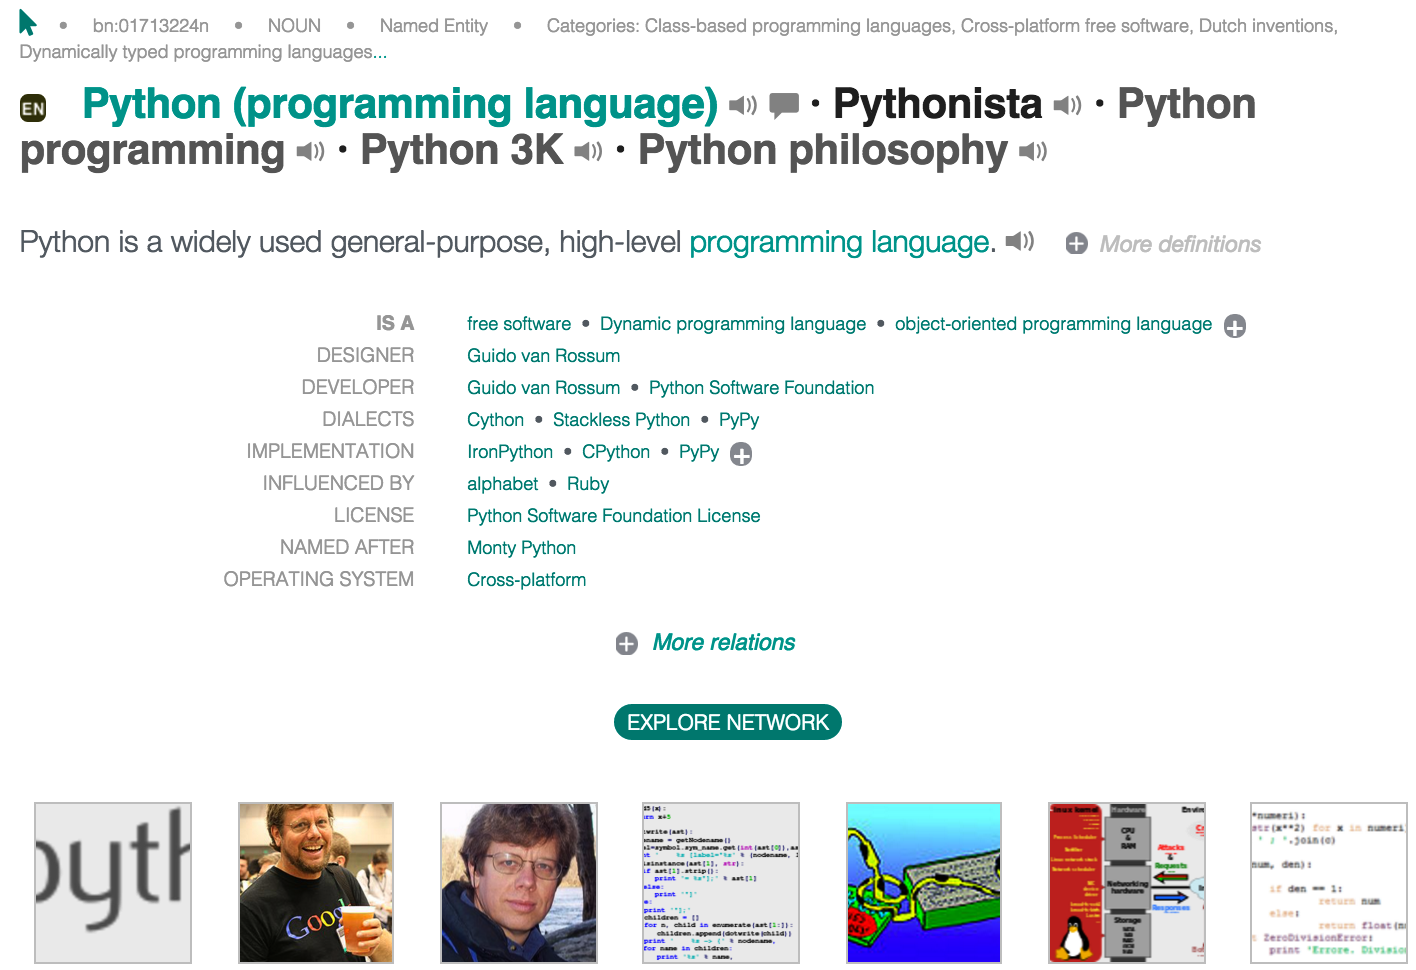
\includegraphics[width=0.49\textwidth]{figures/babelnet}

	\end{center}
	\caption{ BabelNet synset \texttt{ \small bn:01713224n} that corresponds to the  word ``python" in the programming language sense. Definitions, synonyms, taxonomic relations and images make this representation easily interpretable. }
	\label{fig:synset}
\end{figure}


\subsection{Word Sense Embeddings: AdaGram }

The training objective of the Skip-gram model~\cite{mikolov2013efficient} is to find vector word representations that are useful for predicting the surrounding words in a sentence or document. The model represents a word sense as a low-dimensional vector. AdaGram~\cite{bartunov2015breaking} is a Bayesian nonparametric extension of the Skip-gram model that learns several embeddings per word corresponding to word senses. 
 
We chosen AdaGram for experiments as they outperform the approach of Neelakantan et al.~\shortcite{neelakantanefficient} according to several word sense disambiguation benchmarks and have an open source implementation in contrast to the method of Li and Jurafsky~\shortcite{li2015multi}. Few other approaches have important limitations, so we did not consider them either. For instance, the method of Tian et al.~\shortcite{tianEtAl2014} assumes a fixed number of senses for all words, which is undesirable due to exponential distribution of number of senses. The approach of Huang et al.~\shortcite{Huang2012} performs offline clustering of word contexts and thus is computationally expensive for large corpora. On the other hand, AdaGram can be considered as an online clustering of contexts, which therefore can scale to large corpora keeping a reasonable memory footprint. It is scalable due to an online variational learning algorithm used for training. As opposed to \cite{tianEtAl2014}, the number of prototypes is found automatically, while senses granularity is regulated by the resolution parameter $\alpha$.  

As opposed to the interpretable BabelNet representation illustrated in Figure~\ref{fig:synset}, an embedding is a dense vector typically in a 100-500 dimensional space, where the meaning of the dimensions is not specified in any human-interpretable format. The vectors themselves are therefore uninterpretable by humans. 

However, one can interpret a sense vector by comparing it to other vectors. Namely, a list of nearest neighbours in the vector space can be used to interpret a sense. For instance, ten nearest neighbours of the vector corresponding to the word ``python" in the programming language sense obtained during our experiments is as following: ``perl, php, java, smalltalk, ruby, lua, tcl, scripting, javascript, bindings". While in some cases, this list of related words can be sufficient for interpretation of a word sense, it does not contains the wealth of additional information present in BabelNet synsets, such as taxonomic relations, human-readable definitions, images, and so on.   

 
 

For the purpose of this paper, we have trained\footnote{https://github.com/sbos/AdaGram.jl} an AdaGram model on an English corpus consisting of Web documents and Wikipedia articles with the default meta-parameters. Namely the resolution parameter $\alpha$ was set to $0.05$,  yielding 4.2 senses per word in average, and the number of dimensions in sense vectors was set to 100. The choice of the default parameters is dictated by the goal of our experiment. The idea was to show feasibility of linking  two resources, rather than finding an optimal granularity for such alignment. In particular, we used surface forms of ukWaC and WaCkypedia\_EN corpora by Baroni et al.~\shortcite{baroni2009wacky}.\footnote{http://wacky.sslmit.unibo.it/doku.php?id=corpora}

\subsection{Comparison of AdaGram and BabelNet Word Sense Inventories}

There are often considerably more BabelNet senses than AdaGram senses. From Figure \ref{fig:sensescomp}, we can observe a huge discrepancy in granularity of their sense inventories. The inventory of the embeddings is coarse-grained, while inventory of the lexical resource is extremely fine-grained. The maximum number of senses in our AdaGram model, controlled by $\alpha$ parameter, is five, while for the BabelNet it reaches up to 200 senses for some words. 

%Lexical resources are indeed often very fine grained that to be useful for applications. This strengthens also your approach as you can remove them.

Inspection revealed that many of these senses are named entities, such as three roller-coasters named ``Python" with BabelNet IDs \texttt{\small bn:00279773n}, \texttt{\small bn:03501078n} and \texttt{\small bn:14645852n}. Some words, like ``pilot" ``angel" or ``gold", have over 100 senses in BabelNet, many representing rare named entities. 

Our technique can be used to tag any word sense embeddings with synsets from any WordNet-like resource, but BabelNet is especially well suited in this context due to its high coverage of different domains, rare senses and multiple languages. The more senses lexical resource contains the higher the probability that an automatically induced sense will be linked to a synset.

\begin{figure}
	\begin{center}
	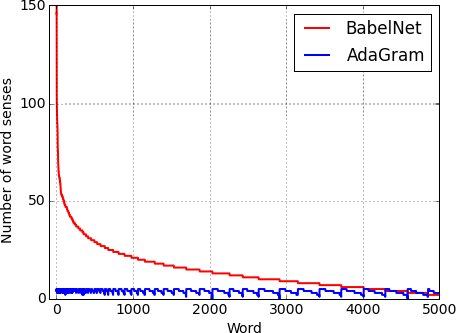
\includegraphics[width=0.5\textwidth]{figures/number-of-senses-150}
	\end{center}
	\caption{ Comparative number of senses in BabelNet and AdaGram for  4724 frequent words.}
	\label{fig:sensescomp}
\end{figure}


\begin{table*}

\footnotesize  
\begin{center}
\begin{tabular}{cccccc}

\bf Word & \bf AdaGram ID & \bf BabelNet ID & \bf Sim. & \bf AdaGram BoW & \bf BabelNet BoW  \\
\hline

python & 2 & bn:01713224n & 0.103   & \parbox{4.6cm}{perl, php, java, smalltalk, ruby, lua, tcl, scripting, javascript, bindings, binding, programming, coldfusion, actionscript, net, $\ldots$} &  \parbox{4.6cm}{ language, programming, pythonista,  python programming, python3, python2, level, computer, pythonistas, python3000, python, $\ldots$ }\\ \hline

python & 1 & bn:01157670n &  0.102  & \parbox{4.6cm}{monty, circus, spamalot, python, magoo, muppet, snoopy, featurette, disney, tunes, tune, classic, shorts, short, apocalypse, $\ldots$} &  \parbox{4.6cm}{monty, comedy, monty python, british, monte, monte python, troupe, pythonesque, foot, artist, record, surreal, terry, $\ldots$ }\\ \hline

python & 3 & bn:00046456n &  0.066  & \parbox{4.6cm}{spectacled, unicornis, snake, giant, caiman, leopard, squirrel, crocodile, horned, cat, mole, elephant, opossum, pheasant, zebra, $\ldots$} &  \parbox{4.6cm}{molurus, indian, boa, tigris, tiger python, rock, tiger, indian python, reptile, python molurus, indian rock python, coluber, bivittatus, $\ldots$ }\\ \hline

python & 4 & bn:01157670n &  0.063  & \parbox{4.6cm}{circus, fly, flying, dusk, lizard, moth, unicorn, puff, adder, vulture, tyrannosaurus, zephyr, badger, $\ldots$} &  \parbox{4.6cm}{monty, comedy, monty python, british, monte, monte python, troupe, pythonesque, foot, artist, record, surreal, terry, $\ldots$ }\\ \hline

python & 1 & bn:00473212n & 0.060   & \parbox{4.6cm}{monty, circus, spamalot, python, magoo, muppet, snoopy, featurette, disney, tunes, tune, classic, shorts, short, apocalypse, $\ldots$} &  \parbox{4.6cm}{pictures, monty, python monty pictures, limited, company, python pictures limited, kingdom, picture, serve, director, united, five, $\ldots$}\\ \hline

python & 1 & bn:03489893n &  0.056  & \parbox{4.6cm}{monty, circus, spamalot, python, magoo, muppet, snoopy, featurette, disney, tunes, tune, classic, shorts, short, apocalypse, $\ldots$} &  \parbox{4.6cm}{film, horror, movie, clabaugh, richard, monster, century, direct, snake, python movie, television, giant, natural, language, for-tv, $\ldots$ }\\ \hline



\end{tabular}
\end{center}
\caption{ Result of the mapping of the AdaGram sense embeddings to the BabelNet synsets for the word ``python" with the threshold of 0.05. The AdaGram BoW contains top nearest neighbours in the vectors space, while the BabelNet BoW contains most frequent words from synset, related words and glosses. This mapping helps to interpret sense vectors linking them to human-understandable synsets available by the BabelNet ID (c.f. Figure~\ref{fig:synset}). }
\label{tbl:example}
\end{table*}
 
 
\section{Linking Embeddings to Synsets}
\label{sec:match}

Our matching technique takes as input a trained word sense embeddings model, a set of synsets from a lexical resource and outputs a mapping from sense embeddings to synsets of the lexical resource. The method includes four steps. First, we convert word sense embeddings to a lexicalized representation and perform alignment via word overlap.  Second we build a bag-of-word (BoW) representation of synsets. Third, we build a bag-of-word representation of  sense embeddings. Finally, we measure similarity of senses and link most similar vector-synset pairs. Below we present each step in detail.


\subsection{Representation of Synsets}
\label{sec:representation}

A bag-of-words that represents a synset is constructed of synset words, glosses, categories assigned to the synset and captions of images representing the synset. Glosses, categories and captions are lemmatized and cleaned from stop-words. For morphological analysis in our experiment we rely on SpaCy.\footnote{https://spacy.io} A word in a bag-of-words is weighted with its normalized frequency $w \in [0;1]$: We build frequency dictionary of words coming from synsets, glosses, categories and captions and simply normalize word counts by the largest word count.

\subsection{Representation of Sense Embeddings}

For each sense vector, we build a bag-of-words featuring the 200 most similar words and their lemmas according to the AdaGram model using the built-in function for nearest neighbors computation. Similarity of a sense to its neighbours is used as bag-of-word weight $w \in [0;1]$. 

\subsection{Linking Sense Representations}

We experimented with two strategies that link sense vectors to synsets: the \textit{global threshold} and the \textit{disambiguation}.

\subsubsection{Linking via Global Threshold} Let a word have $n$ synsets and $m$ sense vectors each represented by a bag-of-words.  Then, in the first approach, we would calculate all $n*m$ pairwise similarities between these senses and link pairs with similarity above certain \textit{global threshold} $t$, where $t$ is the same for all words:
$$
match(v_i, s_j) = \left\{
  \begin{array}{l l}
    1 &  \text{if } sim(v_i, s_j) \geq t \\
    0 & \text{otherwise} 
  \end{array} 
$$
Here $sim(v_i, s_j)$ is a similarity score between a bag-of-word  representing a sense vector $v_i$ and a bag-of-word representing  the synset $s_j$. The similarity between bag-of-words is calculated with either \textit{cosine} or \textit{overlap}. The global threshold method enables many-to-many mapping desirable in this context. As exemplified in Table~\ref{tbl:example}, the ``Monty Python" sense of the word ``python" is represented with two sense embeddings (AdaGram IDs 1 and 4) and two synsets (BabelNet IDs \texttt{\small bn:01157670n} and \texttt{\small bn:00473212n}).   

Sample output of the mapping between sense embeddings and synsets of the word ``python" is presented in Table~\ref{tbl:example}. Further examples of linking AdaGram embeddings to BabelNet of 4724 frequent words are available online.\footnote{Result of linking of AdaGram sense embeddings to BabelNet synsets for 4724 frequent words:  https://goo.gl/dN6WSG}

\subsubsection{Linking via Disambiguation}
The second linking approach starts with \textit{disambiguation} of a synset using the corresponding built-in AdaGram function, which performs a Bayesian inference based on the learned model, c.f.~\cite{bartunov2015breaking}. Namely, we pass a list of words from the bag-of-words to this function as context of the target word. 
Next, we decide to link the assigned sense depending on similarity of either \textit{confidence} of disambiguation or \textit{overlap} of the bag-of-words of $v_i$ and $s_j$. Here again we rely on the global threshold $t$ of these similarities, but in the second strategy, one vector is linked to at most one synset. 

\begin{table*}

\footnotesize 
\begin{center}
\begin{tabular}{l}


%\bf word Method  \\
% \hline

\parbox{17cm}{
ant (3$\vert$11),  apache (3$\vert$19),  apollo (3$\vert$28),  apple (4$\vert$15),  atom (2$\vert$19),  bank (4$\vert$29),  bass (5$\vert$19),  blizzard (2$\vert$9),  bosch (3$\vert$5),  brother (4$\vert$24),  canon (5$\vert$18),  capital (4$\vert$28),  cassandra (2$\vert$20),  citizen (4$\vert$7),  cloud (4$\vert$24),  cobra (3$\vert$34),  commercial (5$\vert$10),  corvette (2$\vert$5),  delphi (2$\vert$10),  focus (5$\vert$38),  jaguar (4$\vert$21),  java (4$\vert$17),  jena (2$\vert$8),  julia (4$\vert$30),  lotus (5$\vert$23),  market (3$\vert$13),  mouse (5$\vert$22),  mustang (4$\vert$13),  network (4$\vert$19),  oracle (4$\vert$25),  organ (5$\vert$11),  pascal (3$\vert$10),  plant (5$\vert$17),  port (4$\vert$25),  puma (3$\vert$19),  python (4$\vert$17),  raspberry (3$\vert$8),  ruby (4$\vert$39),  rust (4$\vert$17),  sex (5$\vert$25),  shell (5$\vert$33),  soul (4$\vert$18),  spark (4$\vert$37),  sphinx (2$\vert$24),  spider (5$\vert$24),  tiger (4$\vert$35),  tomcat (2$\vert$7),  viper (3$\vert$24),  vladimir (3$\vert$11),  word (5$\vert$17)}

\end{tabular}
\end{center}
\caption{ List of ambiguous words used in the evaluation dataset. Here ``ant (3$\vert$11)" denotes that the word ``ant" has 3 AdaGram senses and 11 BabelNet senses. Each word has at least two homonymous senses, e.g. the word ``ant" can denote an insect sense, but also the Java build tool ``Apache Ant".  }
\label{tbl:evaluation}
\end{table*}


\section{Evaluation}

We  evaluate our linking techniques with respect to a manual mapping of senses. In particular, we built an evaluation dataset for 50 ambiguous words  presented in Table~\ref{tbl:evaluation}. More specifically, we selected words with homonymous senses i.e. senses with unrelated meanings, such as ``python" in the animal and the programming language senses. Some of these words, such as ``bank" and ``plant" are commonly used in word sense disambiguation evaluations~\cite{navigli2007semeval,manandhar2010semeval,jurgens2013semeval}; others, like ``delphi" or ``python" may refer to both nouns and named entities.  


For each of these words, we retrieved all BabelNet and AdaGram senses. Next, we generated all 3795 possible matching combinations for these 50 words and annotated them binarily. 


As mentioned above, BabelNet is very fine grained and contains more senses than AdaGram. Word sense embeddings  used in our experiments are on the countrary  coarse-grained with at most five senses per word (this is tunable by the $\alpha$ parameter). Therefore, the corpus-based model cannot learn a fine-grained  polysemic inventory featuring tens of senses. For instance, AdaGram does not contain separate senses for  ``apple fruit"\footnote{http://babelnet.org/synset?word=bn:00005054n} and ``apple fruit as a symbol"\footnote{http://babelnet.org/synset?word=bn:00319426n} found in BabelNet. Instead, it contains senses that correspond to ``apple (computer)" and ``apple (fruit)". That is why, during annotation, we often positively linked a coarse-grained AdaGram sense to a more specific BabelNet sense. The negatively linked senses are those with completely unrelated meanings, such as ``apple" in the company and fruit senses. The final dataset contains 423 positive and 3372 negative sense alignments.\footnote{Evaluation dataset: https://goo.gl/F2kuBA}


\begin{table}

%\small 
\begin{center}
\begin{tabular}{lll}


\bf  Method & \bf BoW Similarity & \bf AUC \\
\hline
random  & random &  0.11 \\ 
disambiguation & confidence & 0.53 \\
disambiguation & overlap & 0.66 \\
global threshold & overlap  & 0.73 \\
%global threshold & cosine & TF-IDF & 0.77 \\
global threshold & cosine & \bf 0.78 \\

\end{tabular}
\end{center}
\caption{ Performance of methods for linking AdaGram sense embeddings to BabelNet synsets on the evaluation dataset of 50 ambiguous words.  }
\label{tbl:auc}
\end{table}

 \begin{figure*}
	\begin{center}
	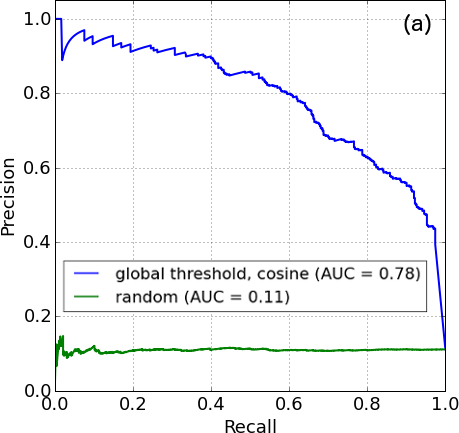
\includegraphics[width=0.41\textwidth]{figures/precision-recall}
	
\includegraphics[width=0.06\textwidth]{figures/filler}
	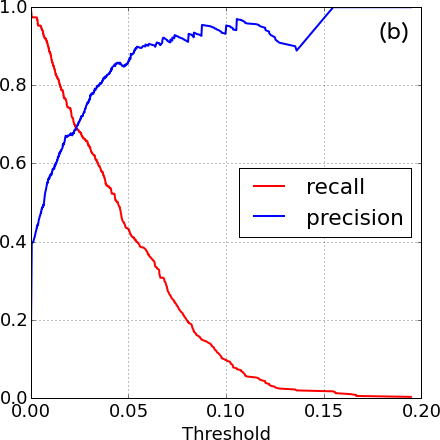
\includegraphics[width=0.40\textwidth]{figures/pr-function-of-threshold}

	\end{center}
\caption{ (a) Precision-recall curve of the best matching method \textit{global threshold cosine} compared to the random mapping. (b) Precision and recall of the the same method function of the threshold $t$.}
	\label{fig:pr}
	
	\end{figure*}

\begin{table}
\centering
\label{my-label}
\begin{tabular}{lllll}
       \bf Class  & \bf Precision & \bf Recall & \bf F-measure & \bf Support \\ \hline
match    & 0.87      & 0.42   & 0.57      & 423     \\
no match & 0.93      & 0.99   & 0.96      & 3372   
\end{tabular}
\caption{Performance of the best linking method \textit{global threshold cosine} on the evaluation dataset of 50 ambiguous words at the threshold value of 0.05.}
\label{tbl:results2}

\end{table}


\section{Results}

Table~\ref{tbl:auc} presents key results of our experiments. The baseline that assigns a random synset to a sense vector has an area under precision-recall curve (AUC) of 0.11.

The matching by built-in AdaGram \textit{disambiguation} sounds attractive, as it relies not only on word overlap, but also on word similarities encoded in the embeddings. Yet, we  observe that it fails for BabelNet senses that have no correspondence in the corpus-induced senses. AdaGram always assigns one of the senses from its inventory, and in such cases provides no meaningful indication of disambiguation confidence. The comparably low AUC of 0.53 of the \textit{disambiguation, confidence} method based on confidence scores of the AdaGram, shows that these scores cannot be used to robustly rank pairs of candidate senses. Using the word overlap instead confidence of disambiguation increases AUC from 0.53 to 0.66. 

According to our experiments, the best way to map senses is simply to calculate cosine between their bag-of-words and then link vector-synset pairs with the similarity above certain threshold. This approach yields an AUC of 0.78 (see also Figure~\ref{fig:pr} (a)). Ranking of sense pairs by overlap provides slightly worse results with AUC of 0.77, showing the utility of similarity scores in this task.

Figure~\ref{fig:pr} (b) depicts dependence of the precision and recall from the threshold value $t$. Precision increases with the value of the threshold and thus a user may select the value that fits best her use-case. For instance, a $t$ value of 0.05 corresponds to precision of 0.87 and recall of 0.42. Table~\ref{tbl:results2} provides a breakdown of the precision and recall scores at the threshold value $t$ of 0.05 for the \textit{global threshold} method using the cosine similarity.  

A relatively low recall of 0.42 at the precision level of 0.87 is caused by two issues. First, some BabelNet synsets have void bag-of-words as no text is associated with their English synset. For instance, the sense \texttt{\small bn:14200967n} of the word ``delphi" and the sense \texttt{\small bn:14944150n} of the word ``java" have no English definitions (this problem may be fixed in future releases). Second, some positive vector-synset pairs are not linked as similarity of their BoW representations is below the threshold $t$ of 0.05. 

For instance, the BabelNet sense of the word ``apple" represented with the bag-of-words ``store, retail, apple store, stores, chain, apple retail store, applestore, boston,... "	has a cosine similarity of 0.002 with the AdaGram vector represented with the BoW ``macintosh, hardware, pc, microsoft, ibm, pcs, dos, emulator, computers, os, beos,...". Yet, both these senses are strongly related. Therefore, a major problem with recall is caused by sparseness of the bag-of-words representation. Prior research \cite{bar2012ukp} suggest that this limitation can be addressed using word relatedness measures. 

% A variation of the global threshold approach is based on \textit{TF-IDF} weighting of sense representations. Here the weighs is calculated in the standard way, but the ``documents" used were all BabelNet and AdaGram senses of a given word. Thus, words specific to certain senses obtained higher weights and words common across senses obtained lower weights.

% Additionally to the configurations reported in Table~\ref{tbl:auc} we tried several other strategies, not presented here due to strictly lower AUC in comparison to the best \textit{global threshold} approach. In particular, we tried to use (1) normalization of BabelNet BoWs by external corpus frequencies; (2) mapping top most similar senses of a given word instead of the global threshold. 





\section{Conclusion}
\label{sec:conc}

Interpretation of clustering results is an inherently difficult problem. Word sense induction via sense embeddings is based on clustering of word contexts and therefore also faces this challenge. We propose a simple yet effective technique that improves interpretability of embeddings by linking them to highly human-readable synsets of a lexical resource, featuring proper definitions, examples of usage, and so on. The approach is able to link up to 42\% of induced senses with precision of 87\%. In addition to interpretability, our approach gives rise to hybrid methods (e.g. word sense disambiguation) that rely on information from both corpora and lexical resources.  

\section{Acknowledgements}

This research was supported by the Deutsche For\-schungs\-gemeinschaft under the project "Joining Ontologies and Semantics Induced from Text" (JOIN-T). Thorough comments of Chris Biemann, Martin Riedl, Benjamin Milde and three anonymous reviewers helped to significantly improve quality of this paper. Besides, I thank Sergey Bartunov for making implementation of the AdaGram available and for explaining how to operate the system. 

\section{Bibliographical References}
\label{main:ref}

\bibliographystyle{lrec2016}
\bibliography{xample}


% \bibliographystylelanguageresource{lrec2016}
% \bibliographylanguageresource{xample}

\end{document}
